\documentclass{article}
\usepackage{graphicx}
\usepackage{enumerate}
\usepackage{setspace}
\usepackage{hyperref}
\usepackage[utf8]{inputenc}
\usepackage[OT1]{fontenc}
\usepackage[french]{babel}
\usepackage{vmargin}
\setpapersize{A4}
\setmargins{15mm}{15mm}{180mm}{260mm}{0pt}{0mm}{0pt}{1.2cm}
\title{Compte rendu OUTILS LIBRES}
\author{REVEL Rémi}
\date{\today}

\begin{document}
\maketitle
\par\noindent\rule{\textwidth}{0.4pt}

 %----------------------------------------DEBUT TD1------------------------------------------
 
\section{\huge{efficatité de l'environnemnt de travail}}

%----------------------------------------Question 1-----------------------------------------------------
\subsection{\large{Desactivation de la souris}}

\subsection*{\normalsize{voici les commande pour desactiver la souris:} } 
\begin{enumerate}
    \item xinput set-prop 4 "Device Enabled" 0

    \item xinput set-prop 6 "Device Enabled" 0

    \item xinput set-prop 7 "Device Enabled" 0
\end{enumerate}

\subsection*{\normalsize{tableau de raccourcis clavier utile:} }    

\begin{center}
   \begin{tabular}{| l | c | }
     \hline
     changer d'application & alt+tab ou windows+tab\\ \hline
     gestionnaire d'application & Touche windows \\ \hline
     Naviguer sur les elements cliquable d'une page web & tab   \\ \hline
     Fermer le navigateur & CTRL+W \\ \hline
     Fermer une appliacation & ALT+F4 \\ \hline
     Changer d'onglet sous Brave & CTRL+1,2,3,...   \\ \hline
     Ouvrir un nouvelle onglet & CMD+T \\ \hline
     faire une recherche & F6 \\ \hline
   \end{tabular}
 \end{center}
 
 %---------------------------------------------------------------------------------------------
 
 %----------------------------------------question 2-----------------------------------------------------
 
 \subsection{\large{S'ameliorer a la dactylographie}}
 le site que j'ai retenu pour s'ameliorer en dactylographie est \href{https://10fastfingers.com/typing-test/french}{10fastfingers}. \par On peut s'entrainer sur des mots aleatoire, ou sur nos propres texte, le site est disponible dans plusieurs langue.

\begin{center}
    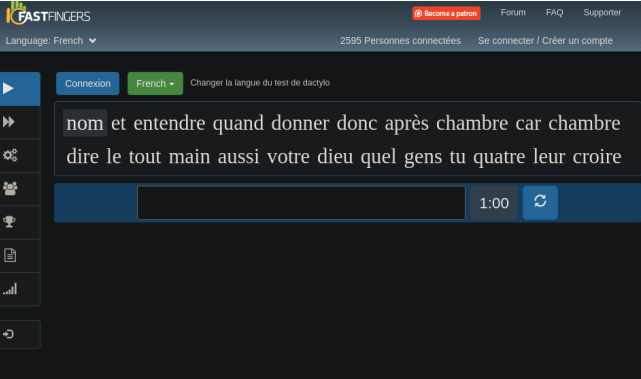
\includegraphics[scale=0.7]{Images/fastfinger.png}
\end{center}

%---------------------------------------------------------------------------------------------

%---------------------------------------------Question 3------------------------------------------------

\subsection{\large{Tutoriel pour VIM}}

\begin{center}
   \begin{tabular}{| l | c | }
     \hline
     insertion & i\\ \hline
     enregister & :w\\ \hline
     quitter & :q \\ \hline
     aller au debut du fichier & :1 \\ \hline
     aller a la fin du fichier & :\textdollar \\ \hline
     annuler une action & u \\ \hline
     recherche d'une occurence & /occurence \\ \hline
     activer coloration syntaxique & :syntax on \\ \hline
     templacer du texte & :s/origin/replacement/g \\ \hline
   \end{tabular}
 \end{center}
 
 pour definir VIM comme editeur par defaut on a juste a rentrer cette commande: \par update-alternatives --set editor /bin/vim
 
 %---------------------------------------------------------------------------------------------
 
 %---------------------------------------------Question 4------------------------------------------------
 
 \subsection{\large{Bash history}}
 
 Mon mot de passe n'apparait pas dans le bash history, donc il n'y a pas d'informations sensible.\par
 Les historiques sont propres a chaque shell utilisé. \\
 
 Pour eviter de poluer notre historique avec des commande basique on peut les exclures avec cette commande : \par
 export HISTIGNORE="ls : cd : pwd"
 
  %---------------------------------------------------------------------------------------------
  
  %---------------------------------------------Question 5------------------------------------------------
  
  \subsection{\large{Alias de fonction}}
  Les commandes presentes ci dessous sont a placer dans le .bashrc
  
  \begin{center}
        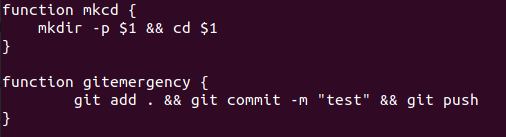
\includegraphics[scale=0.7]{Images/function.png}
  \end{center}
    
 %---------------------------------------------------------------------------------------------
 
 %---------------------------------------------Question 6------------------------------------------------
 
 \subsection{\large{Script}}
 Ce script est fait pour la sauvegarde des données des utilisateurs de la machine.
 
 \begin{center}
        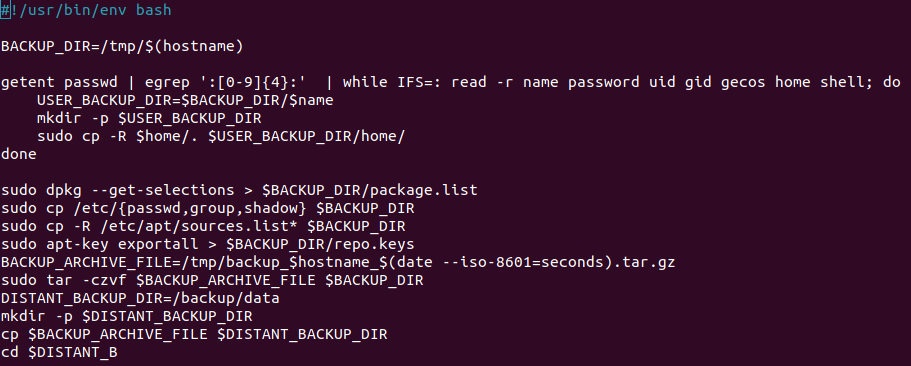
\includegraphics[scale=0.5]{Images/save.png}
 \end{center}
    
 %---------------------------------------------------------------------------------------------
 
 \newpage
 
 %---------------------------------------------Question 7------------------------------------------------
 
 \subsection{\large{customisation avec OH MY ZSH}}
 Dans le fichier du theme oh y zsh que l'on a selectioné on y rajoute ceci pour pouvoir voir le status de nos Vagrant et notre statut git.
 
 \begin{center}
        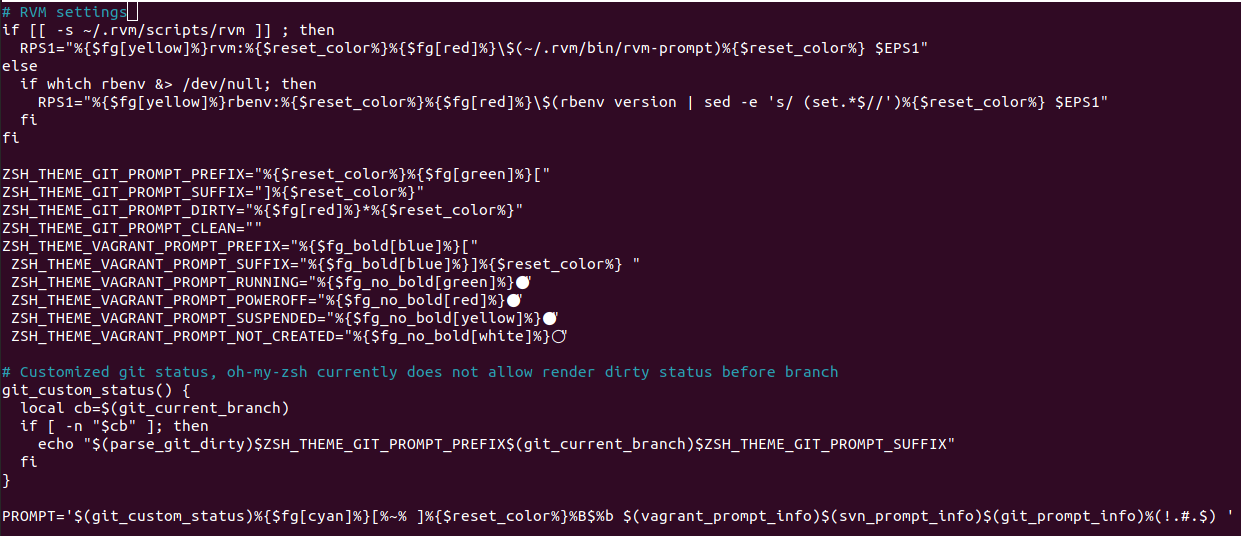
\includegraphics[scale=0.43]{Images/theme.png}
 \end{center}
    
 %---------------------------------------------------------------------------------------------
 
 %---------------------------------------------Question 8------------------------------------------------
 
  \subsection{\large{Raccourci clavier}}
  
  Pour faire un raccourcis clavier qui start ou stop apache en faisant CTRL+A, on place ce petit bout de code dans notre .bashrc
  
  \begin{center}
        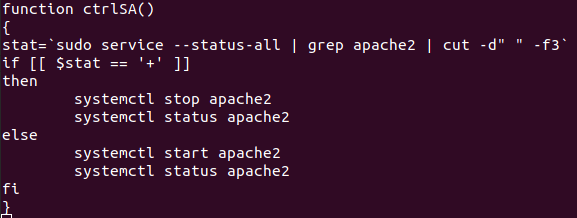
\includegraphics[scale=0.6]{Images/CTRLA.png}
  \end{center}
  
 %---------------------------------------------------------------------------------------------
 
  \newpage
  
 %---------------------------------------------Question 9------------------------------------------------
 
 \subsection{\large{Emulateur de terminaux}}
 
 \subsection*{\normalsize{Sakura :} } 
 C'est un terminal assez simple, il est leger, il fait rien de plus que le terminal qui est present de base sur debian, son avantage un noir profond ce qui fait bien ressortir les couleurs, on a la possibilité d'avoir plusieurs onglets. Couplé au shell fish qui possedent un coloration syntaxique et de l'auto completion basé sur l'historique, ca rend le terminal interessant.
 
 \begin{center}
        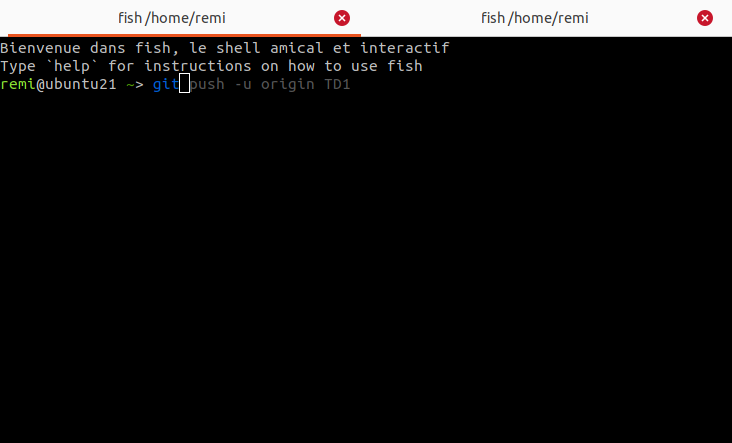
\includegraphics[scale=0.5]{Images/sakura.png}
 \end{center}
 
 \subsection*{\normalsize{urxvt :} } 
 C'est un terminal tres leger, il prend tres peu de ressource, il n'y a pas de possibilité de faire un nouvel onglet. Il est pas tres jolie a voir
 
 \begin{center}
        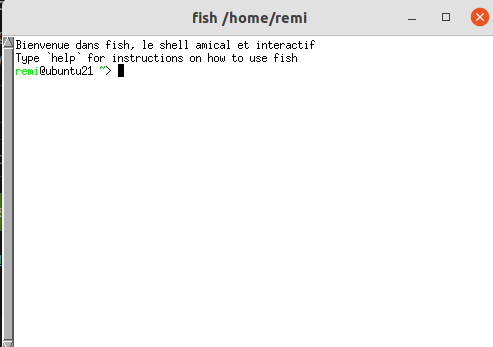
\includegraphics[scale=0.6]{Images/urxvt.png}
 \end{center}
 
 \newpage
  
 \subsection*{\normalsize{Tilix :} } 
C'est un terminal beaucoup plus avancé que les autres, on peut le customiser comme on veut, on peut aussi modifier les raccourcis clavier. Les fenetres de ce terminal peuvent etre logé sous forme de mosaique. Il y a la possibilité que les commandes que l'on tape soit répliqué sur d'autres terminaux. Pour un admin sys, c'est un tres bon terminal.
 
 \begin{center}
        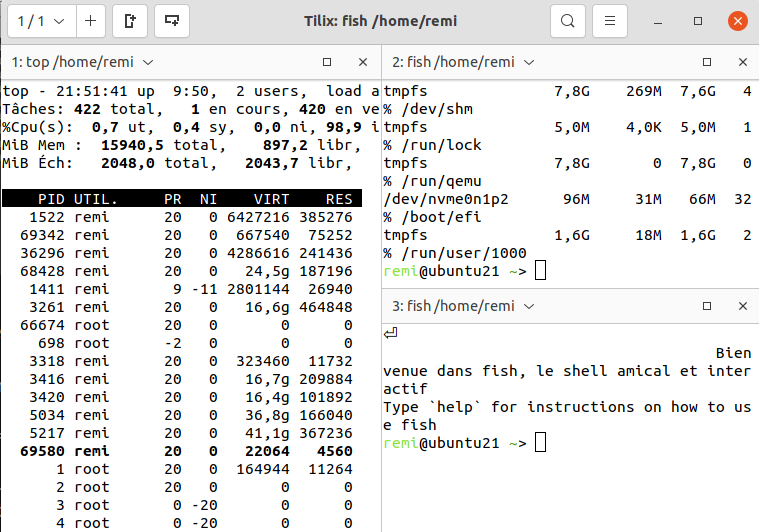
\includegraphics[scale=0.6]{Images/tilix.png}
 \end{center}
 
 %----------------------------------------FIN TD1------------------------------------------
 
 \newpage
 
 %----------------------------------------DEBUT TD2------------------------------------------
 
 \section{\huge{SSH}}
 
 %---------------------------------------------Question 1------------------------------------------------
 
 \subsection{\large{Premiere connection en SSH}}
 Pour se connecter en ssh a srv on entre cette commande: \par sudo ssh carol@10.0.0.3 \par
 on est bien en ssh sur cette machine car ce n'est pas mon ip qui est affiché
 
 \begin{center}
        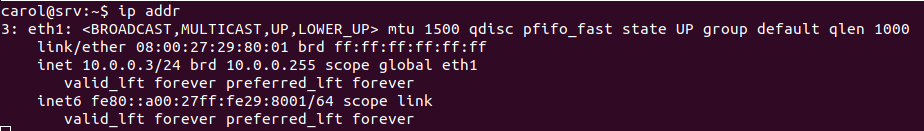
\includegraphics[scale=0.47]{Images/ssh.png}
 \end{center}
 
 %---------------------------------------------Question 1------------------------------------------------
 
 %---------------------------------------------Question 2------------------------------------------------
 
 \subsection{\large{Public key}}
 
 ssh-keygen -b 4096 va nous creer un cle, on lui indique que l'on veut la stocker dans un fichier specifique, dans mon cas le fichier id\_rsa.\par 
 Cette cle une fois crée on la transfert a la machine de destination scp\par
 .ssh/id\_rsa.pub bob@10.0.0.3:./clepub.txt
 il ne reste plus qu'a copié cette cle dans le fichier .ssh/authorized\_keys \par
  cat clepub.txt $>$ .ssh/authorized\_keys
 \\\par
 Une passphrase c’est une phrase qui est demandé lors de notre connection en ssh, elle permet de proteger la clé publique

 %---------------------------------------------Question 2------------------------------------------------
 
 %---------------------------------------------Question 3------------------------------------------------
 
 \subsection{\large{Know host}}
 
 Pour ajouter la clé publique au fichier know host au fichier,il faut taper cette commande: \par
 ssh-keyscan -H 10.0.0.3 $>$ .ssh/known\_hosts
 \\\par
 L'alias de commande pour se connecter a bob avec bs, on configure ca dans le fichier config de ssh
 
 \begin{center}
        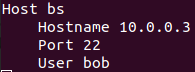
\includegraphics[scale=0.47]{Images/bs.png}
 \end{center}
 
 \begin{center}
        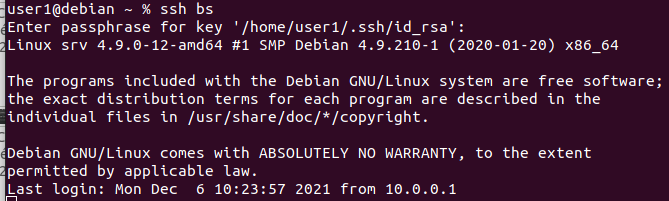
\includegraphics[scale=0.47]{Images/bsresult.png}
 \end{center}
 
 %---------------------------------------------Question 3------------------------------------------------
 
 \newpage
 
 %---------------------------------------------Question 4------------------------------------------------
 
 \subsection{\large{SFTP / SSHFS}}
 
 \subsection*{\normalsize{SFTP} } 
 
 Pour se connecter en sftp a alice c'est la meme syntaxe que ssh mais juste sftp a la place. Il ne reste plus q'ua taper les commande pour transferer des fichier.
 
 \begin{center}
        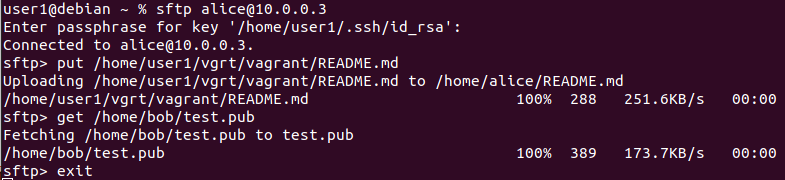
\includegraphics[scale=0.47]{Images/sftp.png}
 \end{center}
  
 on voit bien que les fichier on été transferé
 
 \begin{center}
        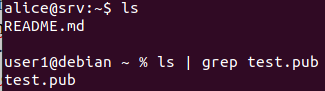
\includegraphics[scale=0.5]{Images/sftpresult.png}
 \end{center}
 
 \subsection*{\normalsize{SSHFS} } 
 
 \begin{center}
        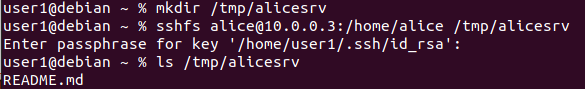
\includegraphics[scale=0.5]{Images/sshfs.png}
 \end{center}
 
 nano /tmp/alicesrv/README.md \par
 j’ai effacé le contenu et mis test a la place
 
 
  \begin{center}
        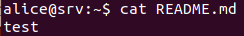
\includegraphics[scale=0.5]{Images/sshfsresult.png}
 \end{center}
 
 %---------------------------------------------Question 4------------------------------------------------
 
 %---------------------------------------------Question 5------------------------------------------------
 
 \subsection{\large{Tunnel SSH}}
 
 Pour se connecter au serveur en passant par cli il faut entrer cette commande, et ne pas quitter le terminal pour \par ne pas fermer la connection. \par
 
 La commande est celle la : ssh -L 8000:10.0.0.3:80 alice@10.0.0.2
 
 ensuite on essaie de voir si on arrive a recuperer un fichier sur le serveur
 
 \begin{center}
        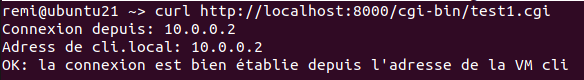
\includegraphics[scale=0.5]{Images/curl.png}
 \end{center}
 
 Si on coupe le tunnel le curl va echouer
 
 \begin{center}
        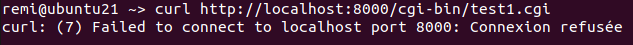
\includegraphics[scale=0.5]{Images/curlfail.png}
 \end{center}
 
 %---------------------------------------------Question 5------------------------------------------------
 
 %---------------------------------------------Question 6------------------------------------------------
 
 \subsection{\large{Tunnel SSH TSOCKS}}
 
 On fait la meme commande qui pour le tunnel ssh mais en changeant de port ssh -L 9000:10.0.0.3:80 alice@10.0.0.2 \par
 
 Sur la machine intermediaire on ouvre le port 9000 : ssh -D 9000 alice@cli.local \par
 
 Pour permetre un SOCKS Proxy sur srv on fait ca : tsocks firefox \par
 
 %---------------------------------------------Question 6------------------------------------------------
 
 \newpage
 
 %---------------------------------------------Question 7------------------------------------------------
 
 \subsection{\large{X11 Forwarding}}
 
 Sur la machine cible on installe x11-apps, ensuite on s'y connecte en ssh avec l'option -x pour le forwarding x11.
 
 \begin{center}
        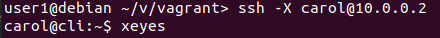
\includegraphics[scale=0.5]{Images/x11.png}
 \end{center}
 
 l'aplication se lance bien sur la cible et s'affiche sur notre poste
 
 \begin{center}
        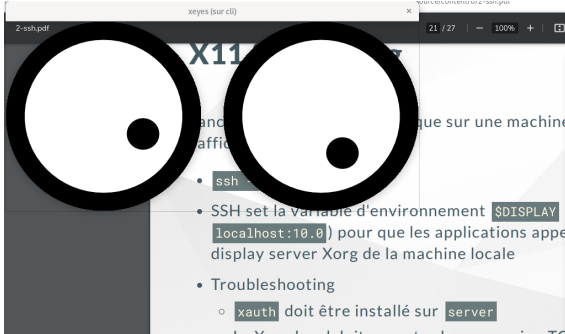
\includegraphics[scale=0.5]{Images/x11result.png}
 \end{center}
 
  %---------------------------------------------Question 7------------------------------------------------
  
  %---------------------------------------------Question 8------------------------------------------------
  
  \subsection{\large{Proxyjump}}
  
  Il faut ajouter dans le fichier config de ssh
  
 \begin{center}
        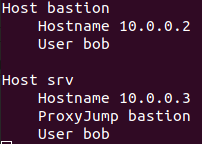
\includegraphics[scale=0.5]{Images/proxyjump.png}
 \end{center}
 
 avec cette methode on ne laise pas de trace sur les machines et c'est plus securisé
 
 %---------------------------------------------Question 8------------------------------------------------
 
 %---------------------------------------------Question 9------------------------------------------------
  
 \subsection{\large{Proxycommand}}
  
  Il faut ajouter dans le fichier config de ssh
  
 \begin{center}
        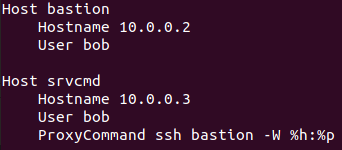
\includegraphics[scale=0.5]{Images/proxycommand.png}
 \end{center}
 
 Cette methode est moins securisé et laisse des traces sur la machine intermediaire 
  
 %---------------------------------------------Question 9------------------------------------------------
 
 \newpage
 
 %---------------------------------------------FIN SSH---------------------------------------------------
 
 
\end{document}
